\documentclass[russian]{vegareport}

\title{Влияние макроэкономических показателей страны на уровень индивидуального благополучия граждан}
\author{Сулейманов Асхаб, Заостровский Всеволод, Черепахин Иван}
\date{}
\usepackage[english,russian]{babel}

\bibliographystyle{nty}

\begin{document}
    \maketitle

    \chapter{Введение}
        \section{Слова и философия}
        В чём смысл существования государства? Этим вопросом задавались тысячи мыслителей на протяжении всей истории человечества. Более того, очень многие из них были твёрдо убеждены в том, что именно им удалось услышать голос Истины, хотя, конечно, сценарий при котором одна и та же Истина, вмещающая в себя сущность государства, одновременно описывается миллионами эпитетов, аллегорий и фразеологизмов, колеблющихся от 'самого холодного из всех холодных чудовищ' до 'намордника для усмирения плотоядного животного, называющегося человеком', кажется, по меньшей мере, весьма и весьма маловероятным. Мы, конечно, не ставим задачи углубиться в тысячелетнюю историю этой дискуссии, и отвечаем на этот вопрос до наивности бесхитростно: смысл государства, равно как и всякого изобретения человечества, состоит в привнесении счастья в печальное настоящее нашего рода.
        \\
        Однако, далеко не все творения покорно следуют замыслам своих создателей, потому интересно разобраться в том, каких побед человечеству удалось достичь на этом поприще и в каком направлении следует двигаться дальше.
        \\
        Конечно, мы далеко не первые люди, которые задались подобными вопросами. Попытки отыскания альтернативных путей для оценки благополучия государств положили начало сравнительно новому направлению экономической теории --- экономике счастья. На данный момент написано весьма впечатляющее число работ, посвященных данной тематике, имеются замечательные результаты, ведётся статистика некоторых показателей.
        \\
        К примеру, сайт \href{https://worldhappiness.report/}{World Happiness Report} встречает своих читателей словами, прекрасно, на наш взгляд, описывающими парадигму этого направления: "our success as countries should be judged by the happiness of our people". В рамках работы, именно \href{https://www.kaggle.com/datasets/mathurinache/world-happiness-report-20152021?select=2016.csv}{их} данные мы будем использовать в качестве меры счастья. Конечно, число подходов к численной оценке индивидуального благополучия ограничено лишь фантазией исследователей и может сильно варьироваться от статьи к статье, в том числе и в исследованиях, ссылки на которые мы даём. Всё же мы считаем, что эти результаты являются серьёзным основанием для построения моделей и интерпретации переменных. Иначе говоря, мы верим в то, что разные определения одного и того же понятия дают схожие результаты.
        \\
        Теперь нам предстоит ответить на очень важный вопрос: "как характеризовать государство и направление в котором оно движется?" Многообразие путей, которые можно избрать для исследования этого аспекта пугающе велико. Есть существенные основания полагать, что счастье имеет социокультурный генезис, поэтому возникает искушение углубиться в этот вопрос в рамках психологической или философской парадигмы. Тем не менее существенным недостатком этого подхода является сложность или невозможность формализации и дальнейшего количественного исследования результатов. Мы будем рассматривать исключительно объективные и измеримые показатели, по которым принято судить о развитости экономики государства, а также те, что могут существенно влиять на самоощущение его граждан.

        \section{Данные}
        В настоящей работе для анализа характеристик стран на макроуровне используются данные Всемирного Банка за 2015-2019 годы. В частности, оттуда была получена следующая информация\footnote{Исчерпывающее техническое описание данных и они сами могут быть найдены по соответствующим ссылкам}:
        \begin{enumerate} \label{table}
        \item \href{https://data.worldbank.org/indicator/NY.GDP.PCAP.PP.CD}{ВВП по ППС на душу населения.}
        \item \href{https://data.worldbank.org/indicator/GB.XPD.RSDV.GD.ZS?view=chart}{Уровень безработицы.}
        \item \href{https://data.worldbank.org/indicator/IC.TAX.TOTL.CP.ZS?view=chart}{Налоговая нагрузка физических лиц.}
        \item \href{https://data.worldbank.org/indicator/FP.CPI.TOTL.ZG?view=chart}{Инфляция.}
        \item \href{https://data.worldbank.org/indicator/SH.XPD.CHEX.GD.ZS}{Государственные расходы на медицину.}
        \item \href{https://data.worldbank.org/indicator/SE.XPD.TOTL.GD.ZS?view=chart }{Государственные расходы на образование.}
        \item \href{https://data.worldbank.org/indicator/MS.MIL.XPND.GD.ZS}{Государственные военные расходы.}
        \item \href{https://data.worldbank.org/indicator/NY.GNS.ICTR.ZS?view=chart}{Валовая экономия.}
        \item \href{https://data.worldbank.org/indicator/SP.POP.DPND}{Демографическая нагрузка.}
        \item \href{https://data.worldbank.org/indicator/VC.IHR.PSRC.P5}{Число убийств на тысячу человек.}
        \end{enumerate}
        В связи с пандемией, данные за 2020 год могли быть значительно искажены, чем и обусловлено решение об исключении этого года из выборки. Что касается более ранних лет, многие необходимые нам статистические данные начали собираться лишь в 2015 году. Не по всем странам обязательно есть наблюдения за каждый год. Более того, для некоторых стран нам не удалось найти информации о критически важных для нашего исследования показателей --- такие страны пришлось исключить из рассмотрения. Здесь используется несбалансированная выборка, с предположением о том, что включение или выбытие страны страны из выборки определяется факторами случайного характера и потому не должно повлечь за собой существенных изменений коэффициентов регрессии. В дальнейшем мы сформировали на их основе несколько моделей, речь о которых пойдёт в следующей главе.

    \chapter{Модели}
        \section{Обзор существующих исследований} \label{review}
        Как отмечалось во введении, экономика счастья --- это весьма популярное направление исследований. Классиком этой области знаний считается Richard Easterlin, обративший внимание в статье \ref{Easterlin} на связь доходов и счастья людей. Долгое время исследователь продвигал идею того, что уровень счастья людей не зависит от их доходов.
        \\
        Однако, в этом вопросе всё не так однозначно. В 2010 году лауреаты премии Нобеля по экономике, Daniel Kahneman1 и Angus Deaton, опубликовали исследование \ref{KahnemanDeaton}, в котором, на примере США, показали, что счастье растёт вместе с доходами до определённого уровня, после которого рост, по меньшеё мере, очень существенно замедляется. Этот вопрос на самом деле невероятно важен и очень неочевиден, потому нам кажется целесообразным включение ВВП в той или иной форме в любые модели предсказания счастья. Впрочем, похоже, что это вполне соответствует общепринятому подходу к моделированию счастья: например, в \ref{DiTella} отмечалась важность роли ВВП. Этот показатель является регрессором в обеих рассматриваемых моделях. Причём, регрессию мы будем строить для логарифма подушевого ВВП по ППС, чтобы учесть эффект, описанный в начале настоящего абзаца.
        \\
        Уровень безработицы также является одним из наиболее классических индикаторов положения дел в государстве. К тому же, есть серьёзные основания полагать, что он должен влиять на чувство удовлетворённости человека. Вопрос связи счастья и безработицы представляет самостоятельный интерес, поэтому существует немало статей, исследующих это, например, в публикации \ref{Winkelmann} было показано, что высокий уровень безработицы негативно влияет на счастье. В статье \ref{Clarkunemp} этот тезис уже называется "общепринятым", сама публикация посвящена исследованию некоторых деталей описываемого явления, кроме того, в ней можно найти ссылки на ещё большее число работ, всесторонне рассматривающих вопрос связи счастья и безработицы.
        \\
        Что касается налоговой нагрузки, то здесь она, с одной стороны, является индикатором активности государственной социальной политики, а с другой, на самом деле может влиять на уровень счастья. Например, в статье \ref{tax} рассмотрена ситуация, в которой доказано влияние подоходного налога на уровень счастья.
        \\
        С инфляцией всё гораздо менее очевидно. С одной стороны, не вызывает сомнений негативное отношение людей к инфляции (причины этого феномена исследуются, например, в статье \ref{Inflation}). С другой стороны, \href{http://www.centralbanknews.info/p/inflation-targets.html}{центральные банки огромного количества стран осуществляют политику таргетирования инфляции}, так что её величина является следствием положения дел в экономике, а не причиной. Счастье же населения, в данном контексте, зависит лишь от того, насколько грамотны решения регулятора. Тем не менее это очень значимый экономический показатель, поэтому мы включаем его в наши модели.
        \\
        Следующая категория объясняющих переменных связана со структурой государственного бюджета в двух наиболее значимых социальных сферах: в медицине (\ref{medicine}) и в образовании (\ref{Education}).
        \\
        Последняя категория переменных была внесена в рассмотрение в попытке описания как можно более разнообразных черт экономического и социального положения государства. Это преследует цель снижения эндогенности модели. Кроме того, мы рассматриваем решение о включении этих переменных в модель как попытку обнаружения новых показателей, значимо влияющих на уровень счастья.

        \section{Модель с 'классическими' объясняющими переменными}
        Целевой параметр описывается уравнением:
        \begin{align*}
        Happiness = \beta_0 + \beta_1 \lg{GDP} + \beta_2 Unemployment + \beta_3 Tax + \beta_4 Inflation + \beta_5 Medicine + \beta_6 Education
        \end{align*}

        Здесь $\lg{GDP}$ --- логарифм ВВП по ППС; $Unemployment$ --- уровень безработицы; $Tax$ -- налоговая нагрузка физических лиц. $Inflation$ --- инфляция; $Medicine$ --- государственные расходы на медицину; $Education$ --- государственные расходы на образование \footnote{см. \ref{table}}.
        \\
        Эта модель построена исходя из "рекомендаций" других статей. К тому же, каждую из переменных принято ассоциировать со счастьем, насчёт каждой из переменных проводились отдельные исследования.


        \section{Модель со 'всеми' переменными}
        Целевой параметр описывается уравнением:
        \begin{align*}
        Happiness = \beta_0 + \beta_1 \lg{GDP} + \beta_2 Unemployment + \beta_3 Tax + \beta_4 Inflation + \beta_5 Medicine + \beta_6 Education \\
            + \beta_7 Military + \beta_8 Savings + \beta_{9} AgeRatio + \beta_{10} Homicides + \beta_{11} Fertility
        \end{align*}

        Здесь $\lg{GDP}$ --- логарифм ВВП по ППС; $Unemployment$ --- уровень безработицы; $Tax$ -- налоговая нагрузка физических лиц. $Inflation$ --- инфляция; $Medicine$ --- государственные расходы на медицину; $Education$ --- государственные расходы на образование; $Military$ --- государственные военные расходы; $Savings$ --- валовая экономия; $Patents$ --- число зарегистрированных патентов по отношению к населению государства; $AgeRatio$ --- демографическая нагрузка; $Homicides$ --- число убийств на тысячу человек \footnote{см. \ref{table}}.
        \\
        В этой версии модели мы попытались рассмотреть как можно более разнообразные метрики благополучия страны.
    
    
    \chapter{Результаты и их интерпретация}
        Результаты регрессионного анализа в рамках двух описанных выше моделей представлены в таблице 3.1 Они вполне предсказуемы: значимого эффекта у переменных вне рамок первой модели обнаружено не было, направление же влияния показателей на уровень счастья согласуется с результатами исследований (\ref{review}). При этом, добавление новых переменных не привело к измению коэффициентов при объясняющих переменных и их уровней значимости.
        \begin{figure}			
            \centering
            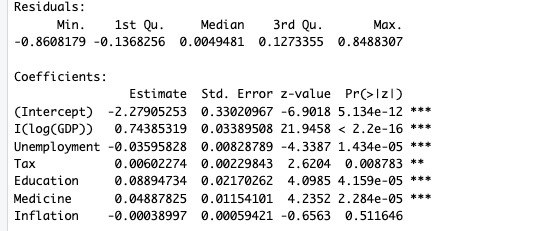
\includegraphics[scale=0.9]{Report/table 2.jpg}
		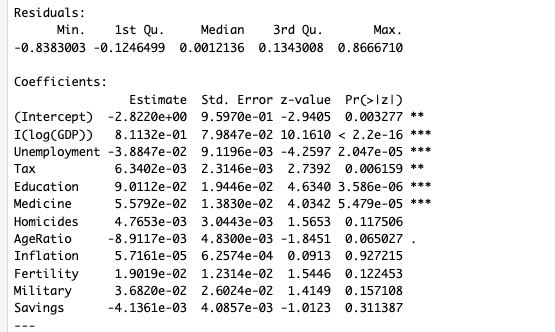
\includegraphics[scale=0.9]{Report/table 1.jpg}
		\caption{Результаты оценивания регрессии оценки уровня счастья WHR для двух спецификаций основной модели}
            \label{lect02:pic1}
	\end{figure}
        \\
        В результатах оценивания регрессии просматривается несколько интересных деталей. Во-первых, не было обнаружено значимого явления инфляции на счастье. Отсутствие связи между этими показателями неочевидно и является довольно ценным аргументом в пользу рассуждений, высказанных в \ref{review}.
        \\
        Во-вторых, не было обнаружено значимого влияния числа убийств (мы считаем это мерой криминализованности общества). С одной стороны, это может показаться странным, с другой же, известно, что, во-первых, больших проблем с учётом убийств не избежали даже развитые страны, а, во-вторых, в менее развитых странах, где криминогенная ситуация гораздо более тревожна, со сбором статистики подобного рода возникают очень существенные трудности, из-за чего de jure показатели развивающихся стран приближаются к de facto показателям развитых. Похоже, что такой эффект, в самом деле, может иметь место(см. рисунок \ref{hompic}).
        \\
        В-третьих, не было обнаружено значимого влияния доли военных расходов на уровень счастья. Это довольно примечательно, поскольку и рассуждения в духе 'высокие траты на оборону укрепляют в гражданах чувство безопасности и величия страны' и таковые из серии 'военные траты есть, в сущности, сожжение денег, нужных для спасения жизней, во имя уничтожения таковых в неугодных государствах, такое мало кого может обрадовать' кажутся довольно здравыми. Не исключено, впрочем, что оба эффекта имеют место и компенсируют друг друга. 
        \\
                \begin{figure} \label{hompic}	
            \centering
            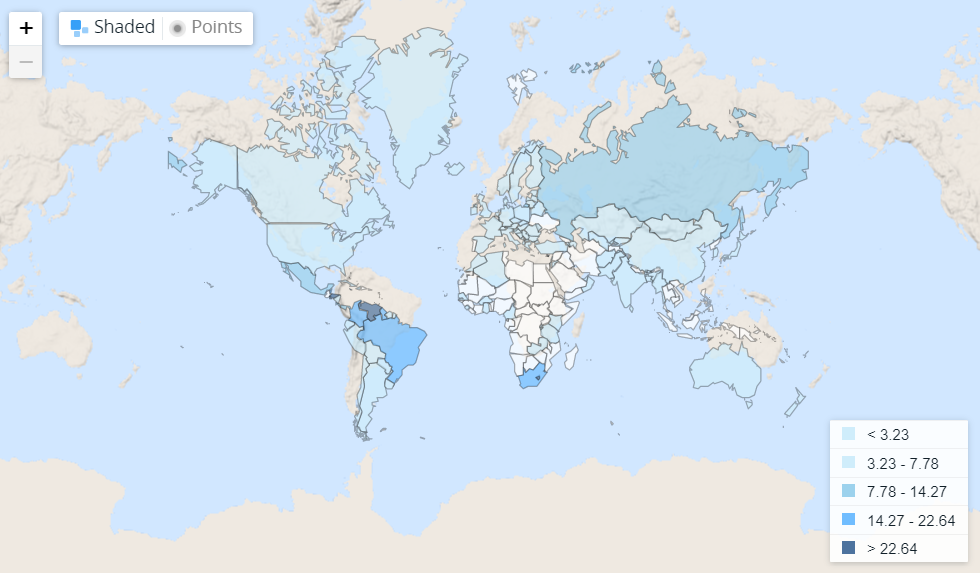
\includegraphics[scale=0.45]{Report/homicides.png}
		\caption{Число убийств на 100000 человек за 2015 год --- данные Всемирного Банка)}
            \label{lect02:pic1}
	\end{figure}
        Что касается незначимости остальных факторов, пожалуй, примечательной была бы ситуация их значимости. Они были добавлены в модель исключительно с целью проверки очевидных соображений и для лучшей эндогенности модели. Это небесполезно, ибо последние нередко оказываются не такими уж очевидными.
        \\
        Как уже отмечалось выше, значимые коэффициенты не преподнесли сюрпризов. Примечательно, что коэффициент при доле трат на образование в два раза превосходит таковой при тратах на медицину. Впрочем, похоже, что это связано с тем, что доля образованых расходов повсеместно меньше (см рисунок \ref{meded}).
        \\
        Также примечательно, что увеличние налоговой нагрузки увеличивает уровень счастья в обществе. Этот эффект свидетельствует в пользу того, что современные государства перераспределяют налоговые поступления довольно эффективно. Однако, стоит отметить, что такой эффект может быть вызван тем, что наиболее счастливыми в мире считаются страны 'скандинавского социализма', для которых характерна высокая налоговая нагрузка.
        
        \begin{figure} \label{meded}			
            \centering
            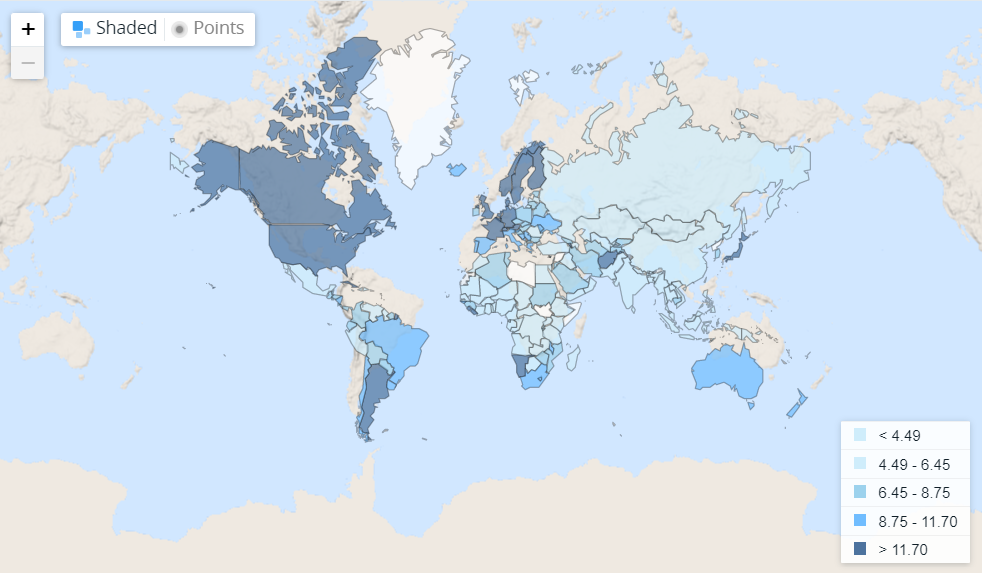
\includegraphics[scale=0.5]{Report/meded1.png}
		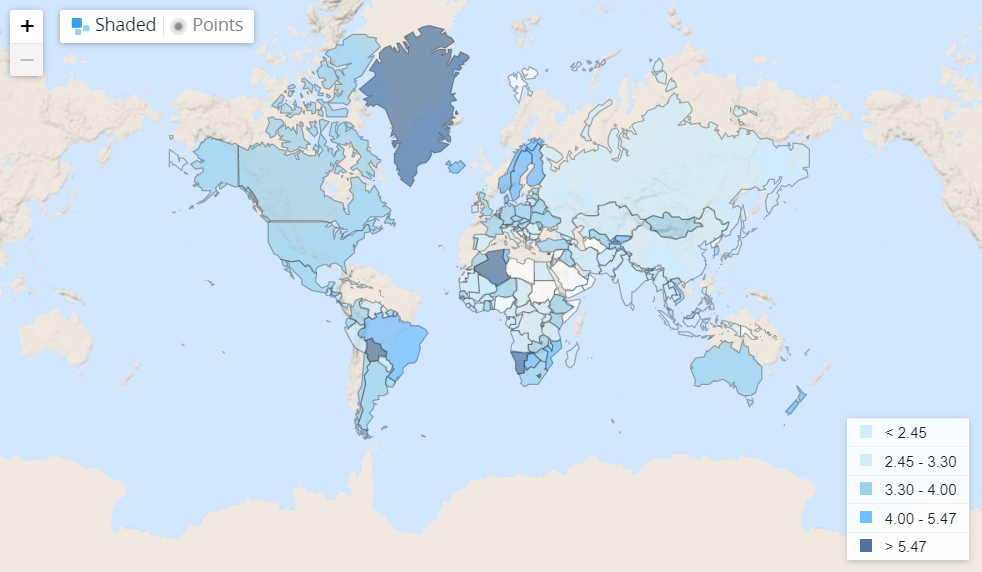
\includegraphics[scale=0.5]{Report/meded2.png}
		\caption{Доля трат в государственном бюджете на медицину и образование, соответственно, за 2015 год}
            \label{lect02:pic1}
	\end{figure}

    
    \chapter{Выводы}
        В статье исследуются две модели, описывающие зависимость счастья от некоторых макроэкономических показателей. Исследования подобных моделей помогают искать ответ на вопрос об этой связи и, на основании этого, строить рекомендации по осуществлению государственной политики и подтверждать (или опровергать) общепринятые идеи.
        \\
        Из ключевых результатов работы можно выделить следующее:
        \begin{itemize}
            \item Общепринятые и очевидные факты: экономическое развитие страны и увеличение доли бюджетных трат на образование увеличивают счастье граждан, увеличение же безработицы его уменьшает --- были подтверждены. Кроме того, были даны ссылки на исследования, более подробно исследующие эти темы.
            \item Увеличние налогов значимо увеличивает уровень счастья в модели.  
            \item Не было выявлено значимого влияния инфляции, доли военных трат и демографической нагрузки на счастье.
            \item Не было выявлено значимого влияния числа убийств на счастье. Впрочем, похоже, что это свидетельствует о несостоятельности этой метрики, а не об отсутствии подобной связи. 
        \end{itemize}
        

    \begin{thebibliography}{100}
            \bibitem{} \label{Easterlin}
            Easterlin R. A.
            Does Economic Growth Improve the Human Lot? Some Empirical Evidence.
            --- \textit{Nations and Households in Economic Growth}, 
            89-125, 1974.

            \bibitem{} \label{KahnemanDeaton}
            Kahneman D., Deaton A. 
            High income improves evaluation of life but not emotional well-being. 
            --- \textit{Proc Natl Acad Sci USA},
            \textbf{38}, 2010.

            \bibitem{} \label{DiTella}
            Di Tella R., MacCulloch R. J., Oswald A. J.
            The macroeconomics of happiness. 
           --- \textit{Review of Economics and Statistics}, 
            \textbf{85}, 1999. 

            \bibitem{} \label{Easterlin2}
            Easterlin R. A.
            Will Raising the Incomes of All Increase the Happiness of All?
            --- \textit{Journal of Economic Behaviour and Organization},
            \textbf{27}, 35-48, 1999. 

            \bibitem{} \label{Clark}
            Clark A. E., Oswald A. J.
            Unhappiness and Unemployment.
            --- \textit{Economic Journal}, 
            \textbf{104}, 648-659, 1994. 

            \bibitem{} \label{Winkelmann}
            Winkelmann L, Winkelmann R.
            Why are the unemployed so unhappy?
            --- \textit{Economica}, 
            \textbf{65}, 1-15, 1998. 

            \bibitem{} \label{tax}
            Hutchinson T., Ahmed I., Buryi P.
            Impact of income tax on happiness: evidence from the United States. 
            --- \textit{Applied Economics Letters}, 1-3.
            1-3, 2016.

            \bibitem{} \label{Clarkunemp}
            Clark A. E.
            A Note on Unhappiness and Unemployment Duration.
            --- \textit{IZA Discussion Paper No. 2406}, 
            2006. 
            
            \bibitem{} \label{Inflation}
            Shiller J. R.
            Why Do People Dislike Inflation?
            --- \textit{NBER Working Paper}, 
            \textbf{5539}, 1996. 

            \bibitem{} \label{medicine}
            Dfarhud D., Maryam M., Khanahmadi M. 
            Happiness & Health: The Biological Factors-Systematic Review Article.
            --- \textit{Iranian Journal of Public Health}, 
            \textbf{43}, 1468-1477, 2014. 

            \bibitem{} \label{Education}
            Satoshi Araki.
            Does Education Make People Happy? Spotlighting the Overlooked Societal Condition.
            --- \textit{Journal of Happiness Studies}, 
            \textbf{23}, 587-629, 2021. 
        \end{thebibliography}


\end{document}